\documentclass[10pt,a4paper]{article}
\usepackage[utf8]{inputenc}
\usepackage{amsmath}
\usepackage{amsfonts}
\usepackage{amssymb}
\usepackage{graphicx}
\usepackage[left=2cm,right=2cm,top=2cm,bottom=2cm]{geometry}

\begin{document}
\section{Understanding the Requirements}



The goal of this project is to implement a Python bytecode interpreter which is engine dependent and also can be hosted on a variety of browsers. So the high level picture of how we have implemented is shown below.

\begin{figure}[ht!]
\center
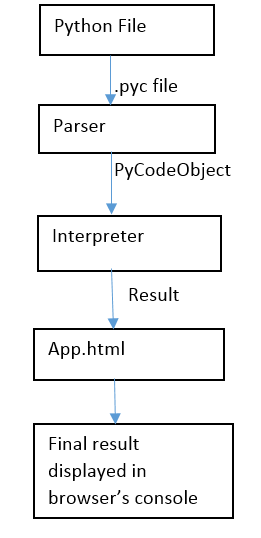
\includegraphics[scale=1]{../Report/UnderstandingTheReq.png} 

\end{figure}
\end{document}


\section{Parser}
